\begin{frame}{Domain knowledge}
In this section, tools and domain knowledges used in the task and reasons of choosing them  will be briefly explained including models used (logistic regression, linear perceptron, XGBoost), evaluation metrices 
(micro-f1, macro-f1) and visualisations (confusion matrix, normalised confusion matrix).
\end{frame}


\begin{frame} {Comparison of Models: Linear Perceptron}
\textbf{Linear Perceptron} is a very simple model for binary classification. After each data are multiplied by weights and biases, the result (scalars) will be passed to the activation function. In the case of unit-step function as the activation function, numbers larger than 0 will be assigned to a class, and vice versa. The whole process can be summarised by the flow chart below.\footnote{https://deepai.org/machine-learning-glossary-and-terms/perceptron}
\begin{figure}[H]
    \centering
    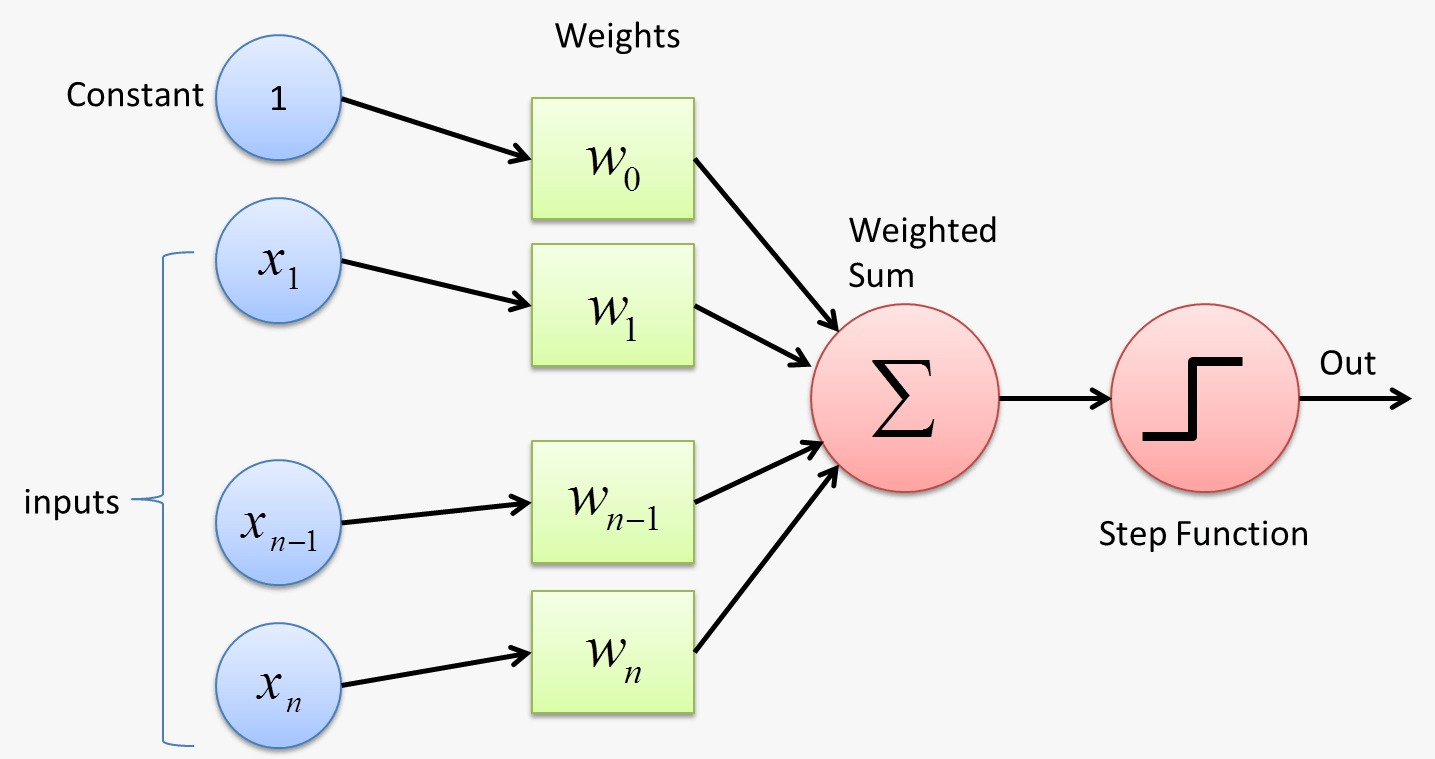
\includegraphics[width=0.7\linewidth]{images/illustrate/linearp.jpeg}
\end{figure}
\end{frame}

\begin{frame} {Comparison of Models: Linear Perceptron}
\textbf{Pros}:
\begin{itemize}
\item Fast and easy to implement; 
\item Less susceptible to overfitting in dealing with small datasets.
\end{itemize}
\textbf{Cons}:
\begin{itemize}
\item High sensitivity to outliers; 
\item Limitations of linearity decision surface nature; 
\item Non-multicollinearity between independent variables needed;
\item Binary outputs only and no calibrated probabilities possible.
\end{itemize}
\end{frame}


\begin{frame}{Comparison of Models: Logistic regression}
\textbf{Logistic regression} is a linear model commonly used for classification problems as well. It is very similar to the linear perceptron model except for the activation function. The activation function for logistic regression is Sigmoid function. For logistic regression, regularisation terms are also added to the loss function as a penalty for overfitting.
\textbf{Pros}: 
\begin{itemize}
\item Regularisation terms helps prevent overfitting;
\item Continuous probabilities for outputs allowed thanks to Sigmoid function.
\end{itemize}
\textbf{Cons}: 
\begin{itemize}
\item Sensitive to outliers;
\item Multicollinearity not allowed.
\end{itemize}
\end{frame}


\begin{frame}{Comparison of Models: XGBoost}
\textbf{XGBoost} is a gradient boosting model with extra structures that has been proved well performed on classification tasks. The boosting model creates weak learner (decision tree) one by one. The previous weak learner set a larger weight for the wrong answers as the input to the next weak learner. By going through the sequence, the classification will eventually be finalised correctly. Each weak learner will have their own predictions, and together they will have to vote to decide what the final answer is. The less accurate weak learners get less votes.
\textbf{Pros}: 
\begin{itemize}
\item Good at tackling non-linear problems; 
\item Non-multicollinearity on data not required; 
\item High efficiency due to the parallel tree boosting and less parameters to be trained.
\end{itemize}
\textbf{Cons}: 
\begin{itemize}
\item High chances of overfitting due to its greediness, but can be solved by setting the correct maximum depth of the trees.
\end{itemize}
\end{frame}

\begin{frame} {Evaluation: Metrics}
Since it is a classification task, f1-score is commonly used for model evaluation. However, f1-score is only calculated per class. 
The multi-class case will require the aggregation of f1-scores of each class to determine the overall performance of the models on all classes. In this case we use Micro-f1 and macro-f1.\\[10pt]
F1-score is defined as equation \autoref{eq:f1_score}.
\begin{equation}\label{eq:f1_score}
	\begin{split}
		\text{f1-score} &= 2\times \frac{\text{precision} \times \text{recall}}{\text{precision} + \text{recall}}\\
		&= \frac{\text{TP}}{\text{TP}+\frac{1}{2}(\text{FP+FN})}
	\end{split}
\end{equation}
\end{frame} 

\begin{frame} {Evaluation: Metrics}
Macro-f1 calculates the average of f1-scores of all classes as equation \autoref{eq:macro_f1}.
The equation shows that macro-f1 \textbf{gives same weights to each class no matter how large the class is}. 
\begin{equation}\label{eq:macro_f1}
	\text{macro-f1} = \frac{\text{sum(f1-score)}}{\text{number of classes}}
\end{equation}
\end{frame} 

\begin{frame} {Evaluation: Metrics}
On the other hand, micro-f1 is defined by equation \autoref{eq:micro_f1}. This equation is the same as the one for f1-score (\autoref{eq:f1_score}). However, the TP, FP and FN stands for the sum of the metrices for all classes. It gives \textbf{equal weights to each data points, resulting in the results dominated by the performance of large classes}.
\begin{equation}\label{eq:micro_f1}
	\text{micro-f1} = \frac{\text{TP}}{\text{TP}+\frac{1}{2}(\text{FP+FN})}
\end{equation}
\end{frame} 

